\documentclass[a4paper,ngerman]{tui-algo-seminar}
\usepackage{graphicx}
\usepackage{algorithm2e}
\usepackage{booktabs}
\usepackage{tikz}
\usepackage{hyperref}
\usepackage{float}
\usepackage{amsmath}
\usepackage{listings}
\usepackage{totpages}
%%\usepackage[margin=1in]{geometry}
\setlength{\footskip}{13.0pt}
\usepackage{thm-restate}

\usepackage[utf8]{inputenc}

\newcommand{\inhalt}{Thüringer Jugend Einzelmeisterschaft 2024}
\seminar{\inhalt}
\semester{\today}
\title{\inhalt}
\author{Erik Skopp}

\usepackage{fancyhdr}
\pagestyle{fancy}
\fancyhf{}
\nolinenumbers

\begin{document}

\maketitle
\thispagestyle{plain}
\begin{abstract}
    Bericht: \inhalt.\\
    Vom 4. bis zum 7. April fand in Naumburg (Sachsen-Anhalt) die diesjährige Thüringer Jugend-Einzelmeisterschaft im Schach statt. In jeder Altersklasse wurden sieben Runden nach dem Schweizer System ausgetragen. Die Gewinner qualifizieren sich für die Deutsche Einzelmeisterschaft in Willingen.
\end{abstract}


\section{Bericht}

\section{Tabellen}
Alle Tabellen entstammen der Veröffentlichung der Thüringer Schachjugend unter folgender URL \url{https://ed.thsj.de/index.php/them-2024}\footnote{Der LInk wurde am \today ~abgerufen.}

% Auch wenn die Pfade nicht stimmen findet Overleaf die Projekte. Bei GitHub und dem Worfkflow ist das nicht so,
\subsection{Hanna Görlach}
    \subsubsection{Partien}
        \begin{table}[htbp]
\centering
\caption{Turnier Rangliste}
\begin{tabular}{|l|c|l|l|c|c|}
\hline
\multicolumn{6}{|c|}{Partien} \\
\hline
Runde & Farbe & Spieler & Verein & ELO & Ergebnis \\
\hline
1 & W & Grube, Anna (2.5) & ESV Lok Meiningen & 841 & 1 \\
2 & S & Brauer, Celiene (4) & SC Turm Erfurt & 1172 & 0.5 \\
3 & S & Ignatova, Gabriela (4.5) & Meuselwitzer SV & 1464 & 0.5 \\
4 & W & Richter, Amélie Elsa (4) & SG Blau-Weiß Stadtilm & 1205 & 0 \\
5 & W & Huth, Fabienne (4) & VfL 1990 Gera & 1072 & 0.5 \\
6 & S & Zeughardt, Selma (3) & Erfurter SK & 1006 & 0.5 \\
7 & W & Scheiding, Sophia (4.5) & Meuselwitzer SV & 1470 & 0 \\
\hline
\multicolumn{4}{|r|}{Gesamt} & Ø 1175 & 3.0 / 5, 13. Platz \\
\hline
\end{tabular}
\end{table}

\section{Bilder}
Bitte keine Bilder von Hanna auf die Website des Ilmenauer SV's\footnote{\url{https:ilmenauer-schachverein.de}} hochladen.
\vspace{0.5cm}
Alle Bilder finden Sie in der Cloud. Bitte nutzen Sie diese. Wir haben von Norbert Reichel via E-Mail die Rechte die Bilder für die Berichte zu nutzen. \\
Die Berechtigung liegt ab dem 19.04 dem Vorstand des Ilmenauer Schachvereines (Markus Hartung) vor.f
    \subsubsection{Rangliste U18w}
        Hier Tabelle einfügen
\subsection{Kashvi Ray}
    \subsubsection{Partien}
        \begin{table}
\begin{tabular}{|c|c|l|l|c|}
\hline
\textbf{Partien} & \textbf{Runde} & \textbf{Spieler} & \textbf{Verein} & \textbf{Punkte} \\ \hline
S & Runde 1 & Ulbrich, Cäcilia (4) & 1. Eichsfelder SC & 1 \\ \hline
S & Runde 2 & Sniegowski, Amalia (6) & Meuselwitzer SV & 0 \\ \hline
W & Runde 3 & Buntin, Amelia Bernadette (5) & ZSG Grün-Weiß Waltershausen & 0 \\ \hline
S & Runde 4 & Nawatzki, Elenor Viktoria (1) & SG Blau-Weiß Stadtilm & 1 \\ \hline
S & Runde 5 & Heß, Julia (3.5) & MTV 1876 Saalfeld & 0 \\ \hline
W & Runde 6 & Nöthlich, Fenja (0.5) & SV Empor Erfurt & 0.5 \\ \hline
S & Runde 7 & Fischer, Emily (2.5) & SV Springer Oldisleben & 0.5 \\ \hline
\multicolumn{4}{|r|}{\textbf{Gesamt (3 Spieler)}} & \textbf{3.0/4} \\ \hline
\multicolumn{4}{|r|}{\textbf{Durchschnitt}} & \textbf{861} \\ \hline
\multicolumn{4}{|r|}{\textbf{Platz}} & \textbf{9.} \\ \hline
\end{tabular}
\caption{Partien Kashvi}
\label{label:Tabelle_Kashvi}
\end{table}
    \subsubsection{Rangliste U10w}
        Hier Tabelle einfügen
\subsection{Ronika Nasiri}
    \subsubsection{Partien}
        \begin{table}[htbp]
\centering
\caption{Turnier Rangliste U12}
\begin{tabular}{|l|c|p{1.8in}|l|c|c|}
\hline
\multicolumn{6}{|c|}{Partien} \\
\hline
\textbf{Runde} & \textbf{Farbe} & \textbf{Spieler} & \textbf{Verein} & \textbf{ELO} & \textbf{Ergebnis} \\
\hline
1 & S & Ulbrich, Eusebia (4.5) & 1. Eichsfelder SC & 810 & 0 \\
2 & S & Weichel, Juliette (3.5) & SV Empor Erfurt & 778 & 0 \\
3 & W & Kührt, Daria (3.5) & SV Empor Erfurt & --- & 1 \\
4 & W & Böttcher, Paulina (2) & SV Springer Oldisleben & 788 & 0 \\
5 & S & Lehmann, Clara Theres (3) & SV Empor Erfurt & 935 & 0 \\
6 & W & Liebaug, Ellen (1.5) & SC Rochade Steinbach-Hallenberg & --- & 1 \\
7 & S & Hoyer, Clara (4) & SV Empor Erfurt & 798 & 0 \\
\hline
\multicolumn{4}{|r|}{Gesamt} & Ø 821 (5 Spieler) & 2.0 / 2, 12. Platz \\
\hline
\end{tabular}
\end{table}
    \subsubsection{Rangliste U12w}
        Hier Tabelle einfügen

\section{Bilder}
\subsection{Bild 1 - Kashvi am Brett}
\begin{center}
    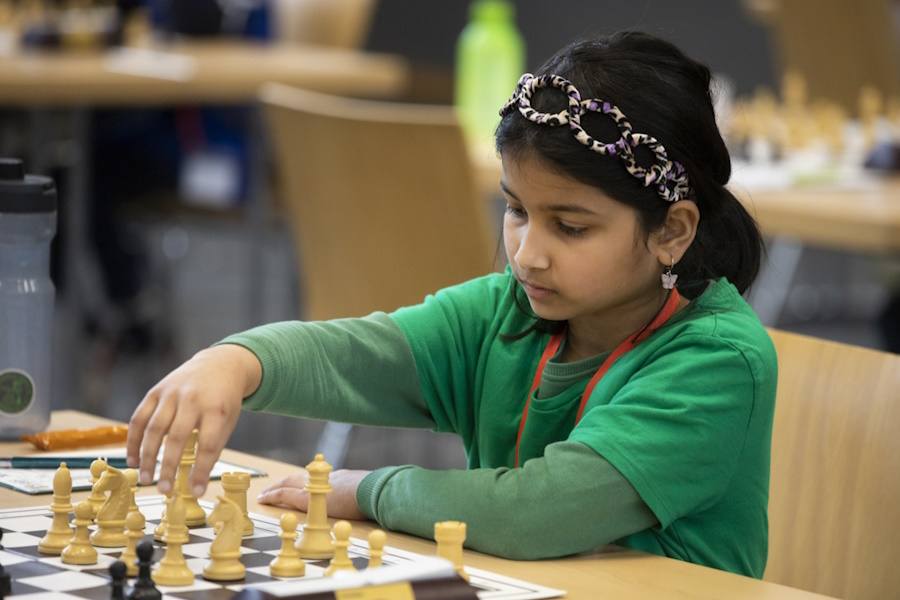
\includegraphics[width=\linewidth,height=0.5625\linewidth,keepaspectratio]{THJEM2.jpg}
    \captionof{figure}{Kashvi Bild}
    \label{fig:Kashvi Bild}
\end{center}

\subsection{Bild 2 - Hanna gegen Anna in Runde 1}
\begin{center}
    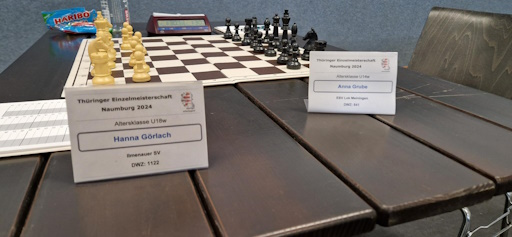
\includegraphics[width=0.8\linewidth,height=0.45\linewidth,keepaspectratio]{THJEM1.jpeg}
    \captionof{figure}{THJEM Hanna Schild}
    \label{fig:THJEM Hanna Schild}
\end{center}




\section{Anmerkungen}




Die Ergebnisse der THJEM 2024 sind, ...
% TODO
\end{document}
